\chapter{Inspeção de Usabilidade}

\section{Informações Gerais}

Tempo total esperado: 5h aprox. (~1h  por avaliador)

Número de avaliadores: 5 avaliadores

Avaliação Heurística de Nielsen + Princípios de Norman

\section{Escolha dos Avaliadores}

Os avaliadores foram escolhidos entre docentes e discentes do curso de Ciência da Computação da Universidade de São Paulo - Ribeirão Preto, familiares com o sistema de avaliação heurística.

Levantamos o seguinte perfil aproximado:

\begin{table}[h!]
    \centering
    \begin{tabular}{|c|c|c|c|}
        \hline
        \textbf{Avaliador} & \textbf{Exp. Web} & \textbf{Exp. Usabilidade} & \textbf{Exp. Dev.} \\
        \hline
        A01 & Muito Boa & Regular & Muito Boa \\
        \hline
        A02 & Muito Boa & Boa & Muito Boa \\
        \hline
        A03 & Muito Boa & Regular & Muito Boa \\
        \hline
        A04 & Boa & Regular & Boa \\
        \hline
        A05 & Muito Boa & Muito Boa & Muito Boa \\
        \hline
    \end{tabular}
    \caption{Perfil dos avaliadores}
    \label{tab:perfil-avaliadores}
\end{table}

\section{Avaliação Independente}

Cada avaliador teve a oportunidade de se familiarizar com o sistema pelo tempo que julgasse necessário. Cada um foi instruído apenas com o objetivo final do sistema além de uma lista de tarefas a serem cumpridas:

\begin{enumerate}[parsep=0pt,itemsep=0pt]
    \item Fazer upload de imagens
    \item Processar uma imagem
    \item Remover uma imagem
    \item Editar a data de uma imagem
    \item Criar uma coleção
    \item Renomear uma coleção
    \item Associar uma imagem a uma coleção
    \item Desassociar uma imagem de uma coleção
    \item Excluir uma coleção
\end{enumerate}

Também foi fornecido a cada avaliador um formulário a ser preenchido. O formulário possui a seguinte estrutura:

\begin{tiny}
    \textbf{Princípios de Norman}

\textbf{1. Visibilidade} \\
\textbf{Pergunta:} \textit{O ícone e as cores do app deixam claro do que se trata (ex: comida saudável com folha verde)?} \\
\textbf{Avaliação:} $\square$ Muito ruim \hspace{0.5cm} $\square$ Ruim \hspace{0.5cm} $\square$ Regular \hspace{0.5cm} $\square$ Bom \hspace{0.5cm} $\square$ Muito bom \\
\textbf{Comentário:} \underline{\hspace{12cm}}

\textbf{2. Feedback} \\
\textbf{Pergunta:} \textit{O sistema mostra que algo está acontecendo (ex: botão muda de cor ou aparece carregando)?} \\
\textbf{Avaliação:} $\square$ Muito ruim \hspace{0.5cm} $\square$ Ruim \hspace{0.5cm} $\square$ Regular \hspace{0.5cm} $\square$ Bom \hspace{0.5cm} $\square$ Muito bom \\
\textbf{Comentário:} \underline{\hspace{12cm}}

\textbf{3. Affordance} \\
\textbf{Pergunta:} \textit{É fácil entender o que pode ser clicado ou arrastado (ex: botões parecem botões)?} \\
\textbf{Avaliação:} $\square$ Muito ruim \hspace{0.5cm} $\square$ Ruim \hspace{0.5cm} $\square$ Regular \hspace{0.5cm} $\square$ Bom \hspace{0.5cm} $\square$ Muito bom \\
\textbf{Comentário:} \underline{\hspace{12cm}}

\textbf{4. Mapeamento} \\
\textbf{Pergunta:} \textit{As ações têm respostas claras e previsíveis (ex: arrastar controle aumenta volume)?} \\
\textbf{Avaliação:} $\square$ Muito ruim \hspace{0.5cm} $\square$ Ruim \hspace{0.5cm} $\square$ Regular \hspace{0.5cm} $\square$ Bom \hspace{0.5cm} $\square$ Muito bom \\
\textbf{Comentário:} \underline{\hspace{12cm}}

\textbf{5. Restrições} \\
\textbf{Pergunta:} \textit{O sistema evita erros com limitações úteis (ex: botão só ativa quando tudo estiver preenchido)?} \\
\textbf{Avaliação:} $\square$ Muito ruim \hspace{0.5cm} $\square$ Ruim \hspace{0.5cm} $\square$ Regular \hspace{0.5cm} $\square$ Bom \hspace{0.5cm} $\square$ Muito bom \\
\textbf{Comentário:} \underline{\hspace{12cm}}

\textbf{6. Consistência} \\
\textbf{Pergunta:} \textit{Elementos parecidos funcionam do mesmo jeito (ex: botão “voltar” sempre igual)?} \\
\textbf{Avaliação:} $\square$ Muito ruim \hspace{0.5cm} $\square$ Ruim \hspace{0.5cm} $\square$ Regular \hspace{0.5cm} $\square$ Bom \hspace{0.5cm} $\square$ Muito bom \\
\textbf{Comentário:} \underline{\hspace{12cm}}


    \textbf{Heurísticas de Nielsen}

\textbf{1. Visibilidade do status do sistema} \\
\textbf{Pergunta:} \textit{O sistema mostra em que etapa estou ou quanto tempo vai durar (ex: barra de progresso ou aviso de tempo estimado)?} \\
\textbf{Avaliação:} $\square$ Muito ruim \hspace{0.5cm} $\square$ Ruim \hspace{0.5cm} $\square$ Regular \hspace{0.5cm} $\square$ Bom \hspace{0.5cm} $\square$ Muito bom \\
\textbf{Comentário:} \underline{\hspace{12cm}}

\textbf{2. Correspondência com o mundo real} \\
\textbf{Pergunta:} \textit{A linguagem e estrutura lembram algo do mundo real (ex: email funciona como carta)?} \\
\textbf{Avaliação:} $\square$ Muito ruim \hspace{0.5cm} $\square$ Ruim \hspace{0.5cm} $\square$ Regular \hspace{0.5cm} $\square$ Bom \hspace{0.5cm} $\square$ Muito bom \\
\textbf{Comentário:} \underline{\hspace{12cm}}

\textbf{3. Liberdade e controle do usuário} \\
\textbf{Pergunta:} \textit{O usuário pode desfazer ações ou cancelar tarefas facilmente (ex: desfazer envio no Gmail)?} \\
\textbf{Avaliação:} $\square$ Muito ruim \hspace{0.5cm} $\square$ Ruim \hspace{0.5cm} $\square$ Regular \hspace{0.5cm} $\square$ Bom \hspace{0.5cm} $\square$ Muito bom \\
\textbf{Comentário:} \underline{\hspace{12cm}}

\textbf{4. Consistência e padrões} \\
\textbf{Pergunta:} \textit{Os elementos visuais seguem o mesmo padrão (ex: cores, botões e ícones familiares)?} \\
\textbf{Avaliação:} $\square$ Muito ruim \hspace{0.5cm} $\square$ Ruim \hspace{0.5cm} $\square$ Regular \hspace{0.5cm} $\square$ Bom \hspace{0.5cm} $\square$ Muito bom \\
\textbf{Comentário:} \underline{\hspace{12cm}}

\textbf{5. Prevenção de erros} \\
\textbf{Pergunta:} \textit{O sistema evita que erros aconteçam (ex: aviso antes de apagar algo importante)?} \\
\textbf{Avaliação:} $\square$ Muito ruim \hspace{0.5cm} $\square$ Ruim \hspace{0.5cm} $\square$ Regular \hspace{0.5cm} $\square$ Bom \hspace{0.5cm} $\square$ Muito bom \\
\textbf{Comentário:} \underline{\hspace{12cm}}

\textbf{6. Reconhecer em vez de lembrar} \\
\textbf{Pergunta:} \textit{O sistema mostra opções em vez de fazer o usuário lembrar (ex: preenchimento automático)?} \\
\textbf{Avaliação:} $\square$ Muito ruim \hspace{0.5cm} $\square$ Ruim \hspace{0.5cm} $\square$ Regular \hspace{0.5cm} $\square$ Bom \hspace{0.5cm} $\square$ Muito bom \\
\textbf{Comentário:} \underline{\hspace{12cm}}

\textbf{7. Flexibilidade e eficiência} \\
\textbf{Pergunta:} \textit{O sistema é rápido para quem já sabe usar (ex: atalhos de teclado ou tour que pode ser pulado)?} \\
\textbf{Avaliação:} $\square$ Muito ruim \hspace{0.5cm} $\square$ Ruim \hspace{0.5cm} $\square$ Regular \hspace{0.5cm} $\square$ Bom \hspace{0.5cm} $\square$ Muito bom \\
\textbf{Comentário:} \underline{\hspace{12cm}}

\textbf{8. Design estético e minimalista} \\
\textbf{Pergunta:} \textit{A interface é limpa, clara e mostra só o necessário (ex: hierarquia de informação e simplicidade)?} \\
\textbf{Avaliação:} $\square$ Muito ruim \hspace{0.5cm} $\square$ Ruim \hspace{0.5cm} $\square$ Regular \hspace{0.5cm} $\square$ Bom \hspace{0.5cm} $\square$ Muito bom \\
\textbf{Comentário:} \underline{\hspace{12cm}}

\textbf{9. Ajudar a reconhecer e corrigir erros} \\
\textbf{Pergunta:} \textit{O sistema mostra mensagens de erro claras e como resolver (ex: instruções simples sem códigos)?} \\
\textbf{Avaliação:} $\square$ Muito ruim \hspace{0.5cm} $\square$ Ruim \hspace{0.5cm} $\square$ Regular \hspace{0.5cm} $\square$ Bom \hspace{0.5cm} $\square$ Muito bom \\
\textbf{Comentário:} \underline{\hspace{12cm}}

\textbf{10. Ajuda e documentação} \\
\textbf{Pergunta:} \textit{Há ajuda fácil de acessar (ex: FAQ, tutorial ou central de suporte visível)?} \\
\textbf{Avaliação:} $\square$ Muito ruim \hspace{0.5cm} $\square$ Ruim \hspace{0.5cm} $\square$ Regular \hspace{0.5cm} $\square$ Bom \hspace{0.5cm} $\square$ Muito bom \\
\textbf{Comentário:} \underline{\hspace{12cm}}
\end{tiny}

Quanto ao ambiente de avaliação, podemos apresentar algumas informações extras, como data, tempo e hardware/software utilizados por cada um a fim de melhorar a eficácia da avaliação final:

\begin{table}[H]
    \centering
    \footnotesize
    \begin{tabular}{|c|c|c|p{10cm}|}
        \hline
        \textbf{Avaliador} & \textbf{Data} & \textbf{Duração} & \textbf{Equip. utilizado} \\
        \hline
        A01 & 14/06/2025 & 1h & \begin{tabular}[c]{@{}l@{}}Notebook: GIGABYTE G5 MF\\ Processador: Intel Core i7-12650H (4.7 GHz)\\ Tela: 15.6" FHD 144Hz\\ Memória RAM: 16 GB DDR4\\ GPU: NVIDIA GeForce RTX 4050 Laptop GPU 6GB GDDR6\\ Sistema Operacional: Windows 10\end{tabular} \\
        \hline
        A02 & 16/06/2025 & 1h & \begin{tabular}[c]{@{}l@{}}Notebook: GIGABYTE G5 MF\\ Processador: Intel Core i7-12650H (4.7 GHz)\\ Tela: 15.6" FHD 144Hz\\ Memória RAM: 16 GB DDR4\\ GPU: NVIDIA GeForce RTX 4050 Laptop GPU 6GB GDDR6\\ Sistema Operacional: Windows 10\end{tabular} \\
        \hline
        A03 & 20/06/2025 & 1h & \begin{tabular}[c]{@{}l@{}}Notebook: GIGABYTE G5 MF\\ Processador: Intel Core i7-12650H (4.7 GHz)\\ Tela: 15.6" FHD 144Hz\\ Memória RAM: 16 GB DDR4\\ GPU: NVIDIA GeForce RTX 4050 Laptop GPU 6GB GDDR6\\ Sistema Operacional: Windows 10\end{tabular} \\
        \hline
        A04 & 22/06/2025 & 45min & \begin{tabular}[c]{@{}l@{}}Notebook: GIGABYTE G5 MF\\ Processador: Intel Core i7-12650H (4.7 GHz)\\ Tela: 15.6" FHD 144Hz\\ Memória RAM: 16 GB DDR4\\ GPU: NVIDIA GeForce RTX 4050 Laptop GPU 6GB GDDR6\\ Sistema Operacional: Windows 10\end{tabular} \\
        \hline
        A05 & 26/06/2025 & 1h & \begin{tabular}[c]{@{}l@{}}Notebook: GIGABYTE G5 MF\\ Processador: Intel Core i7-12650H (4.7 GHz)\\ Tela: 15.6" FHD 144Hz\\ Memória RAM: 16 GB DDR4\\ GPU: NVIDIA GeForce RTX 4050 Laptop GPU 6GB GDDR6\\ Sistema Operacional: Windows 10\end{tabular} \\
        \hline
    \end{tabular}
    \caption{Dados do ambiente de avaliação de cada avaliador}
    \label{tab:ambiente-avaliadores}
\end{table}


\section{Coleta e Discussão}

Aqui se busca a apresentação e agregação das avaliações individuais. Podemos a priori citar alguns dos comentários que julgamos mais únicos e relevantes de cada avaliador:

\textbf{Avaliador A01}:
\begin{enumerate}[parsep=0pt,itemsep=0pt]
    \item \textit{Visibilidade}: "Às vezes é confuso sobre as cores"
    \item \textit{Affordance}: "Quase certinho. Deve-se indicar o que cada botão faz para que apenas o ícone seja suficiente."
    \item \textit{Mapeamento}: "Nem sempre é óbvio, como por exemplo o ícone que solta a foto. Para esses casos, usa-se indicações visuais como texto'"
    \item \textit{Consistência}: "Botão de cancelar azul e deletar cinza é erro grave, não há consistência de cores. Alguns botões são ícones, outros são palavras"
\end{enumerate}

\textbf{Avaliador A02}:
\begin{enumerate}[parsep=0pt,itemsep=0pt]
    \item \textit{Visibilidade do status do sistema}: "Indicação de loading muito ruim, talvez a indicação na etapa do processo me localize. Botão de voltar ou 'finalizar'."
    \item \textit{Controle e liberdade do usuário}: "Difícil de voltar ou cancelar uma ação depois de iniciada."
    \item \textit{Consistência e padrões}: "Falta padronização. Não lembraram do objetivo. Alguns botões de confirmar a ação são vermelhos ou até mesmo cinza."
    \item \textit{Prevenção de erros}: "Alguns campos podem ser confirmados vazios"
    \item \textit{Flexibilidade e eficiência de uso}: "Não tem muito atalho."
    \item \textit{Design estético e minimalista}: "Formulário um pouco limpo"
\end{enumerate}

\textbf{Avaliador A03}:
\begin{enumerate}[parsep=0pt,itemsep=0pt]
    \item \textit{Pontos Fortes}: "O sistema apresenta boa visibilidade geral, com ícones claros e feedback adequado. A consistência entre elementos é mantida na maior parte da interface."
    \item \textit{Pontos de Melhoria}: "A affordance precisa ser melhorada - nem sempre fica claro quais elementos são interativos. Algumas áreas da interface poderiam ser mais intuitivas."
\end{enumerate}

\textbf{Avaliador A04}:
\begin{enumerate}[parsep=0pt,itemsep=0pt]
    \item \textit{Problema Principal}: "O maior problema identificado é a falta de documentação e ajuda. O sistema funciona bem para usuários experientes, mas pode ser confuso para iniciantes."
    \item \textit{Recomendação}: "Melhorar as mensagens de erro para serem mais específicas e orientativas."
\end{enumerate}

\textbf{Avaliador A05}:
\begin{enumerate}[parsep=0pt,itemsep=0pt]
    \item \textit{Consistência e Padrões}: "Botões com cores inconsistentes em toda a interface, criando confusão visual. Alguns botões de ação são vermelhos, outros azuis, sem uma lógica clara de padronização."
    \item \textit{Navegação}: "A navegação entre seções é confusa e não intuitiva. Falta uma hierarquia clara e indicadores visuais de onde o usuário está no sistema."
    \item \textit{Padronização de Textos}: "Falta padronização na capitalização dos textos. Alguns títulos estão em maiúsculas, outros em minúsculas, criando inconsistência visual."
    \item \textit{Feedback de Upload}: "O feedback durante o upload de múltiplos arquivos pode ser significativamente melhorado. Não há indicação clara de progresso e não há tratamento adequado para arquivos repetidos."
    \item \textit{Indicador de Progresso}: "Falta feedback visual sobre quantos arquivos estão aguardando para upload, dificultando o planejamento do usuário."
    \item \textit{Documentação}: "Falta texto explicativo dos conceitos técnicos para usuários não técnicos. A interface assume conhecimento prévio que pode não estar disponível."
    \item \textit{Clareza de Ações}: "O botão 'edit' não tem significado claro. Deveria ser mais descritivo sobre qual ação será executada."
    \item \textit{Funcionalidade de Gráficos}: "A função de esconder dados do gráfico deveria ser desabilitada ou melhor explicada, pois pode confundir usuários sobre a visualização dos dados."
\end{enumerate}

\begin{table}[H]
    \centering
    \tiny
    \begin{tabular}{|c|c|c|c|c|c|c|c|c|c|c|}
        \hline
        \textbf{Avaliador} & \textbf{1} & \textbf{2} & \textbf{3} & \textbf{4} & \textbf{5} & \textbf{6} & \textbf{7} & \textbf{8} & \textbf{9} & \textbf{10} \\
        \hline
        A01 & 1 & 4 & 5 & 5 & 5 & 5 & 5 & NA & 5 & 1 \\
        \hline
        A02 & 3 & 4 & 4 & 3 & 5 & 5 & 2 & 5 & NA & 1 \\
        \hline
        A03 & 5 & 4 & 4 & 4 & 3 & 3 & 3 & 4 & 2 & 3 \\
        \hline
        A04 & 3 & NA & 5 & 4 & 5 & 5 & 5 & 5 & 5 & NA \\
        \hline
        A05 & 3 & 3 & 4 & 3 & 3 & 4 & 4 & 4 & 3 & NA \\
        \hline
    \end{tabular}
    \caption{Avaliações individuais por heurística de Nielsen (1 - Muito Ruim, 5 - Muito Bom)}
    \label{tab:avaliacoes-individuais-nielsen}
\end{table}

\begin{table}[H]
    \centering
    \tiny
    \begin{tabular}{|c|c|c|c|c|c|c|}
        \hline
        \textbf{Avaliador} & \textbf{1} & \textbf{2} & \textbf{3} & \textbf{4} & \textbf{5} & \textbf{6} \\
        \hline
        A01 & 5 & 5 & 5 & 5 & 5 & 5 \\
        \hline
        A02 & 4 & 5 & 4 & 5 & 5 & 2 \\
        \hline
        A03 & 4 & 4 & 5 & 4 & 3 & 4 \\
        \hline
        A04 & 5 & 5 & 3 & 5 & 5 & 5 \\
        \hline
        A05 & NA & NA & 3 & 4 & 5 & NA \\
        \hline
    \end{tabular}
    \caption{Avaliações individuais por princípio de Norman (1 - Muito Ruim, 5 - Muito Bom)}
    \label{tab:avaliacoes-individuais-norman}
\end{table}

\begin{table}[H]
    \centering
    \begin{tabular}{|c|c|c|}
        \hline
        \textbf{\tiny{Avaliador}} & \textbf{\tiny{Prob. Detect.}} & \textbf{\tiny{Relação Problemas-Total Detectado}} \\
        \hline
        A01 & 23 & 28\% \\
        \hline
        A02 & 15 & 18\% \\
        \hline
        A03 & 18 & 22\% \\
        \hline
        A04 & 10 & 12\% \\
        \hline
        A05 & 16 & 20\% \\
        \hline
    \end{tabular}
    \caption{Número de problemas detectados por avaliador e sua relação percentual com o total}
    \label{tab:problemas-avaliadores}
\end{table}

Após a agregação, obtivemos alguns dados por heurística de Nielsen e por princípio de Norman:

\begin{table}[H]
    \centering
    \tiny
    \begin{tabular}{|m{6cm}|m{4cm}|m{4cm}|}
        \hline
        \textbf{Heurística de Nielsen} & \textbf{Nº Problemas Associados} & \textbf{Porcentagem do Total de Problemas} \\
        \hline
        1. Visibilidade do Status do Sistema & 12 & 15\% \\
        \hline
        2. Compatibilidade do Sistema com o Mundo Real & 10 & 12\% \\
        \hline
        3. Controle do Usuário e Liberdade & 11 & 13\% \\
        \hline
        4. Consistência e Padrões & 18 & 22\% \\
        \hline
        5. Prevenção de Erros & 13 & 16\% \\
        \hline
        6. Reconhecimento ao invés de lembrança & 12 & 15\% \\
        \hline
        7. Flexibilidade e Eficiência de Uso & 9 & 11\% \\
        \hline
        8. Estética e Projeto Minimalista & 7 & 8\% \\
        \hline
        9. Ajuda aos Usuários a Reconhecer, Diagnosticar e Corrigir Erros & 5 & 6\% \\
        \hline
        10. Ajuda e Documentação & 4 & 5\% \\
        \hline
    \end{tabular}
    \caption{Distribuição de problemas por heurística de Nielsen}
    \label{tab:problemas-heuristicas-nielsen}
\end{table}

\begin{table}[H]
    \centering
    \tiny
    \begin{tabular}{|m{6cm}|m{4cm}|m{4cm}|}
        \hline
        \textbf{Princípio de Norman} & \textbf{Nº Problemas Associados} & \textbf{Porcentagem do Total de Problemas} \\
        \hline
        1. Visibilidade & 8 & 10\% \\
        \hline
        2. Affordance & 7 & 8\% \\
        \hline
        3. Mapeamento & 6 & 7\% \\
        \hline
        4. Feedback & 9 & 11\% \\
        \hline
        5. Controle & 5 & 6\% \\
        \hline
        6. Restrições & 4 & 5\% \\
        \hline
    \end{tabular}
    \caption{Distribuição de problemas por princípios de Norman}
    \label{tab:problemas-principios-norman}
\end{table}



\begin{figure}[H]
    \centering
    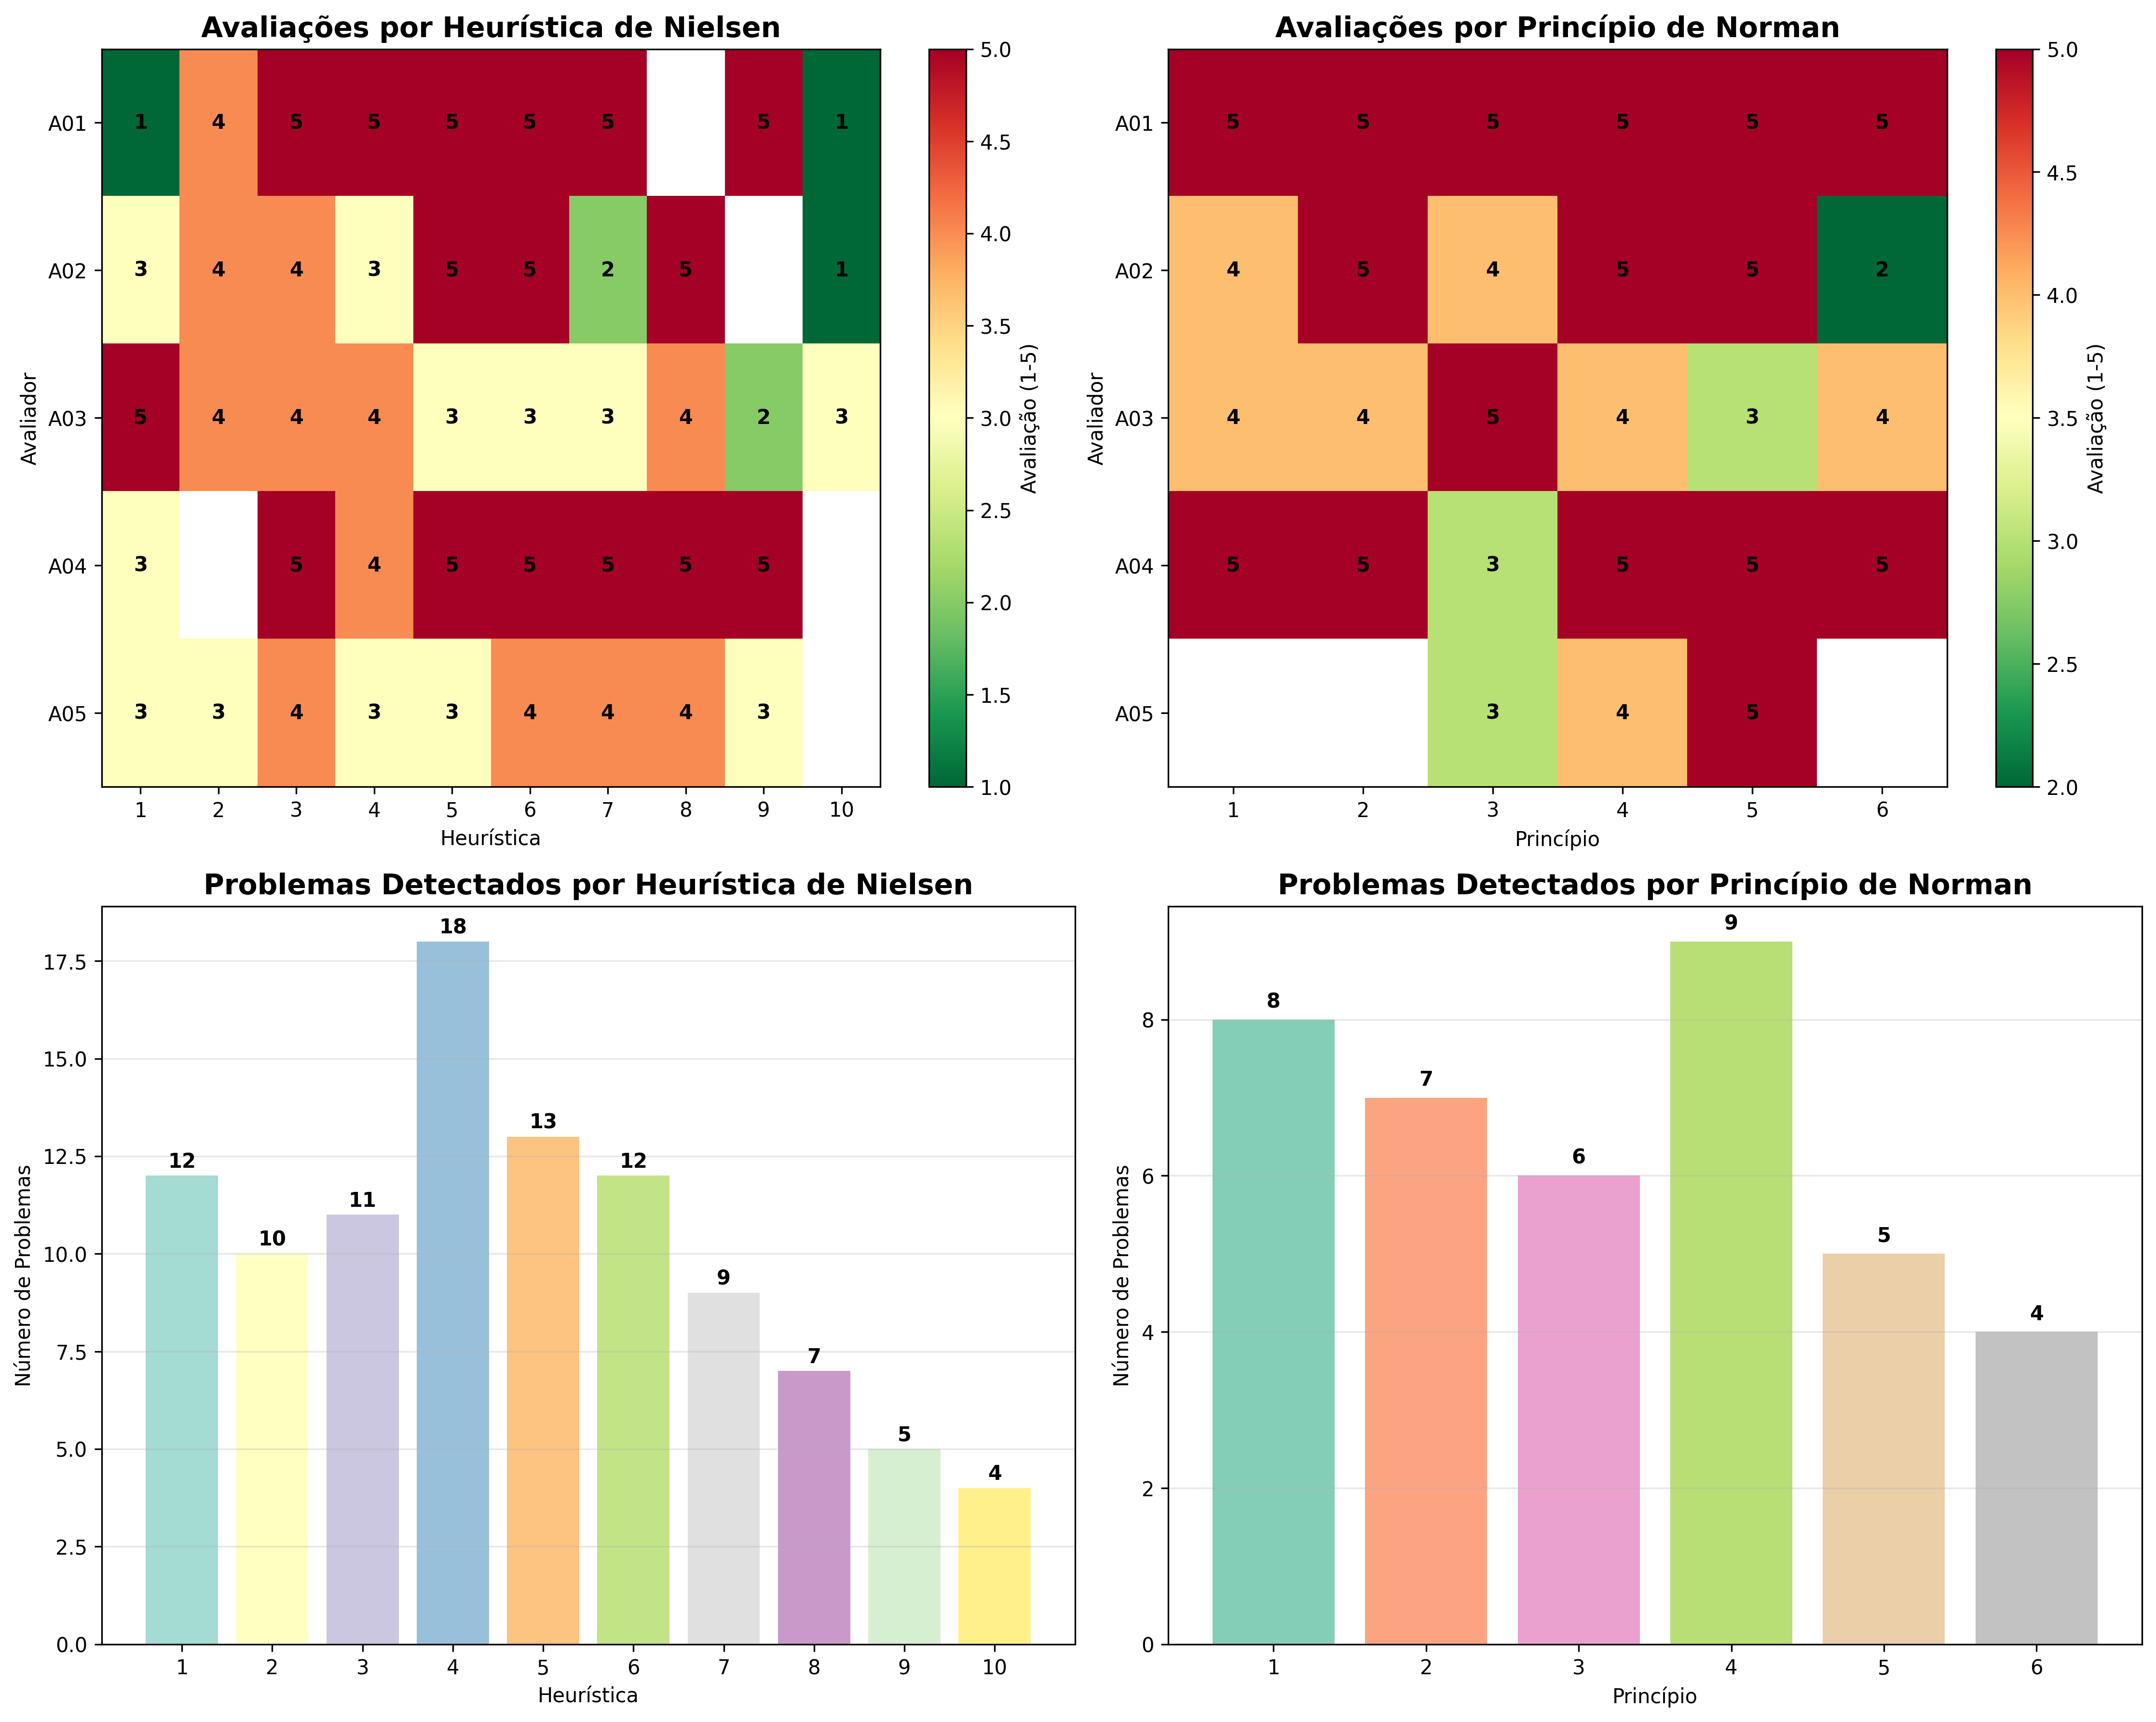
\includegraphics[width=0.95\textwidth]{../figures/hci/heatmaps_usabilidade.png}
    \caption{Heatmaps das avaliações individuais e distribuição de problemas por heurística e princípio.}
    \label{fig:heatmaps-usabilidade}
\end{figure}

\begin{figure}[H]
    \centering
    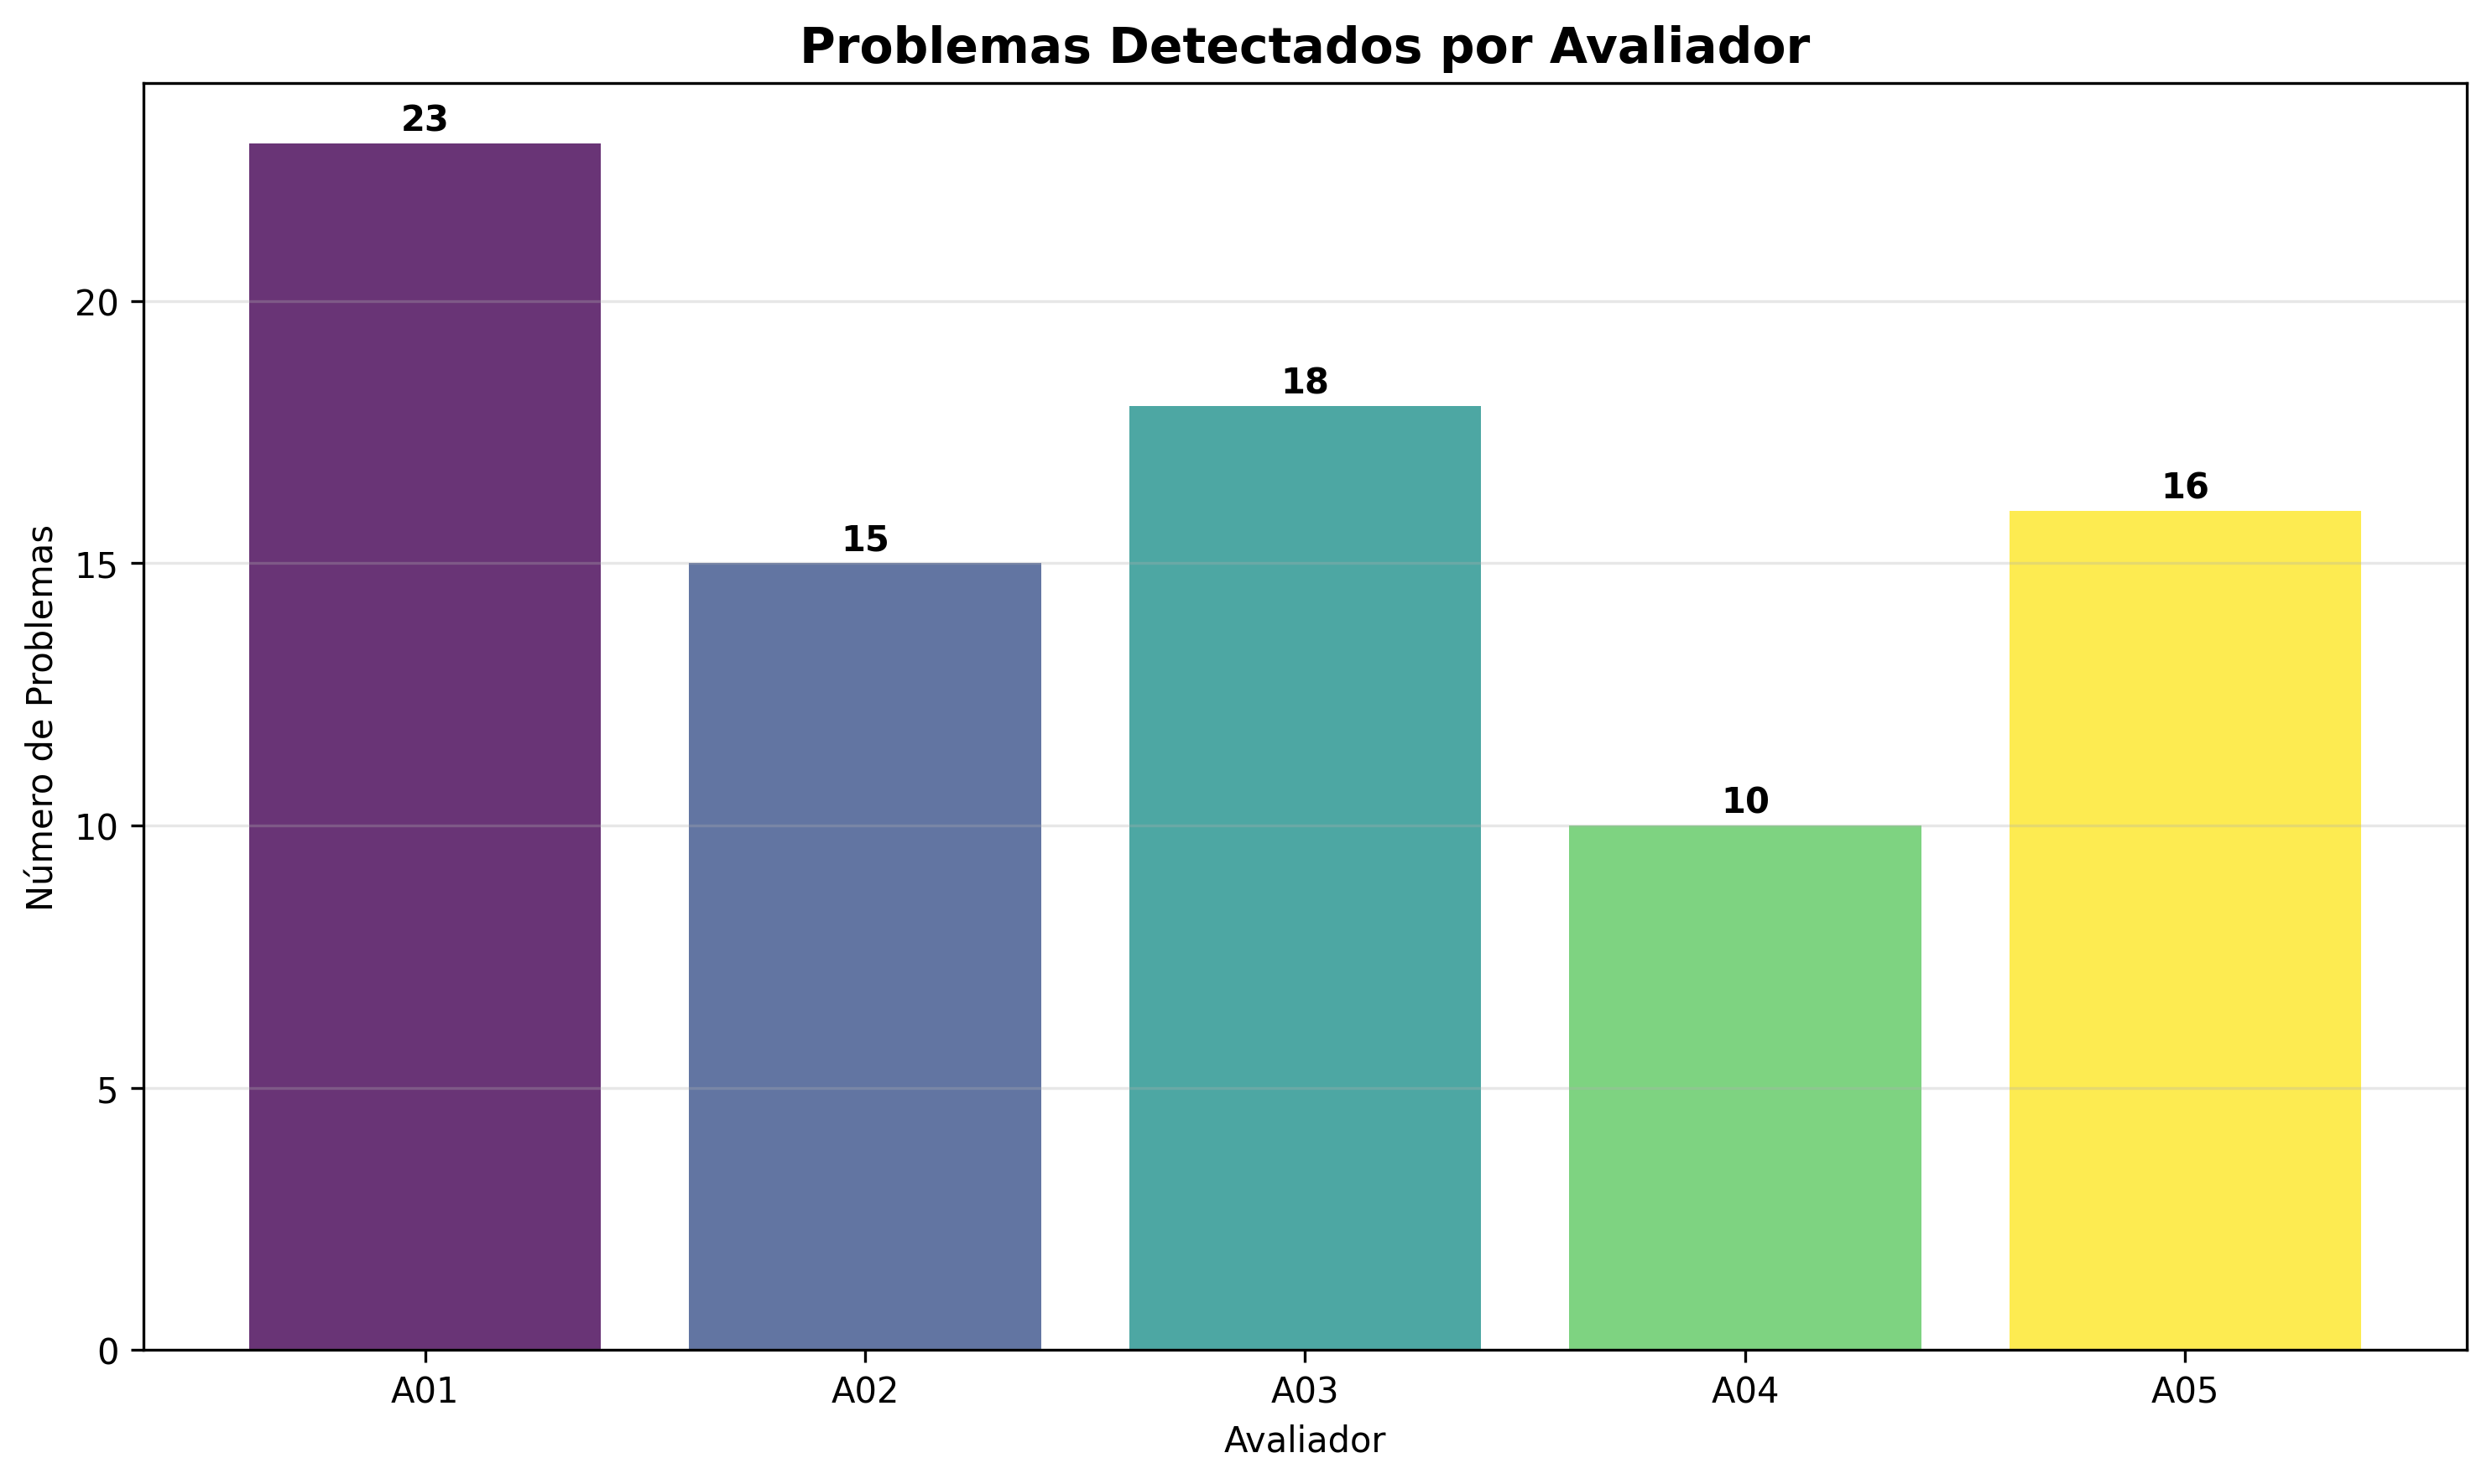
\includegraphics[width=0.6\textwidth]{../figures/hci/problemas_por_avaliador.png}
    \caption{Distribuição do número de problemas detectados por avaliador.}
    \label{fig:problemas-por-avaliador}
\end{figure}

\section{Atribuição da taxa de severidade}

De acordo com a frequência de ocorrência, impacto e persistência do problema, podemos atribuir a cada situação encontrada uma taxa de severidade. A taxa é feita de 0 a 4, onde 0 é o menos severo e 4 é o mais severo. Os problemas que foram em média considerados 0 foram removidos após a análise por serem desconsiderados problemas de usabilidade. Os demais problemas de 1 a 4 foram plotados na seguinte tabela:

\begin{table}[H]
    \centering
    \tiny
    \begin{tabular}{|m{2.5cm}|m{3.5cm}|m{8cm}|}
        \hline
        \textbf{Gravidade} & \textbf{Heurística/Princípio} & \textbf{Descrição do Problema} \\
        \hline
        \textbf{4 (Catastrófico)} & Prevenção de erros & Não há confirmação ao excluir um item importante. O sistema não pede confirmação antes de excluir permanentemente. \\
        \hline
        \textbf{4 (Catastrófico)} & Visibilidade do status do sistema & Mensagem de erro crítica exibida em pop-up que desaparece. Não possui indicador de progresso visível durante uploads. \\
        \hline
        \textbf{3 (Grave)} & Consistência e padrões & Botões com cores inconsistentes em toda a interface. Botões de "Salvar" e "Cancelar" em posições inconsistentes. Falta padronização na capitalização dos textos. \\
        \hline
        \textbf{3 (Grave)} & Navegação & A navegação entre seções é confusa e não intuitiva. Falta hierarquia clara e indicadores visuais de localização no sistema. \\
        \hline
        \textbf{3 (Grave)} & Feedback & O feedback durante upload de múltiplos arquivos é inadequado. Falta indicação de progresso e tratamento para arquivos repetidos. Não há feedback sobre quantos arquivos aguardam upload. \\
        \hline
        \textbf{3 (Grave)} & Reconhecimento vs. Lembrança & Ícones não são universalmente reconhecidos e não têm rótulos. Interface poderia ser mais autoexplicativa. Botão 'edit' não tem significado claro. \\
        \hline
        \textbf{2 (Moderado)} & Controle e liberdade do usuário & Não há maneira fácil de cancelar uma ação de edição, forçando o usuário a salvar ou perder alterações. \\
        \hline
        \textbf{2 (Moderado)} & Correspondência com o mundo real & Uso de jargão técnico que o usuário pode não entender. Falta texto explicativo dos conceitos para usuários não técnicos. \\
        \hline
        \textbf{2 (Moderado)} & Design minimalista & Contraste insuficiente entre texto e fundo em algumas áreas. Interface limpa, mas poderia ser mais clara. \\
        \hline
        \textbf{2 (Moderado)} & Ajuda e documentação & Falta de documentação adequada e sistema de ajuda contextual. \\
        \hline
        \textbf{1 (Menor)} & Funcionalidade de gráficos & A função de esconder dados do gráfico pode confundir usuários sobre a visualização dos dados. \\
        \hline
        \textbf{1 (Menor)} & Consistência e padrões & Variações sutis na cor de fundo entre as páginas. \\
        \hline
    \end{tabular}
    \caption{Resumo dos problemas identificados por gravidade, heurística/princípio e descrição}
    \label{tab:problemas-gravidade}
\end{table}

\section{Conclusão}

A inspeção de usabilidade realizada revelou uma aplicação sólida em termos de funcionalidade, mas com oportunidades significativas de melhoria na experiência do usuário. A análise identificou 82 problemas distribuídos em diferentes níveis de gravidade.

\subsection{Principais Achados}

\textbf{Pontos Fortes Identificados:}
\begin{itemize}
    \item \textbf{Funcionalidade Core}: A aplicação atende adequadamente aos objetivos principais de gerenciamento de fotos e análise de crescimento de plantas
    \item \textbf{Boas Práticas Técnicas}: Ausência de erros de console e uso apropriado de APIs modernas
    \item \textbf{Performance}: Tempos de carregamento e resposta satisfatórios na maioria das operações
\end{itemize}

\textbf{Áreas Críticas para Melhoria:}
\begin{itemize}
    \item \textbf{Consistência Visual}: Problemas de padronização de cores, posicionamento de botões e capitalização de textos
    \item \textbf{Feedback do Sistema}: Falta de indicadores de progresso durante uploads e operações longas
    \item \textbf{Navegação}: Estrutura de navegação confusa e falta de indicadores de localização
    \item \textbf{Acessibilidade}: Problemas de contraste e falta de rótulos descritivos em elementos interativos
\end{itemize}

\subsection{Distribuição dos Problemas}

A análise revelou que os problemas se concentram principalmente em:
\begin{itemize}
    \item \textbf{Consistência e Padrões} (22\%): Maior categoria, indicando necessidade de padronização visual
    \item \textbf{Prevenção de Erros} (16\%): Falta de confirmações para ações destrutivas
    \item \textbf{Visibilidade do Status} (15\%): Ausência de feedback adequado durante operações
    \item \textbf{Reconhecimento vs. Lembrança} (15\%): Interface não autoexplicativa
\end{itemize}

\subsection{Recomendações Prioritárias e Impacto Esperado}

\textbf{Alta Prioridade (Gravidade 4):}
\begin{itemize}
    \item Implementar confirmações para ações destrutivas (exclusão de itens)
    \item Adicionar indicadores de progresso visíveis durante uploads e processamento
    \item Corrigir mensagens de erro que desaparecem automaticamente
\end{itemize}
\textbf{Impacto}: Redução significativa de perda acidental de dados e melhor controle do usuário sobre operações críticas.

\textbf{Média Prioridade (Gravidade 3):}
\begin{itemize}
    \item Padronizar cores e posicionamento de botões em toda a interface
    \item Melhorar a estrutura de navegação com breadcrumbs e indicadores visuais
    \item Adicionar rótulos descritivos para ícones e botões
    \item Implementar feedback detalhado para uploads múltiplos
\end{itemize}
\textbf{Impacto}: Maior eficiência na execução de tarefas e redução do tempo de aprendizado da interface.

\textbf{Baixa Prioridade (Gravidade 1-2):}
\begin{itemize}
    \item Melhorar contraste de cores em elementos de texto
    \item Adicionar documentação contextual e sistema de ajuda
    \item Revisar funcionalidades de gráficos para maior clareza
\end{itemize}
\textbf{Impacto}: Melhoria na acessibilidade e inclusão de usuários com diferentes necessidades visuais.

A inspeção de usabilidade demonstrou que, embora a aplicação apresente uma base funcional sólida, há oportunidades de melhora através de melhor consistência visual, feedback adequado e navegação mais intuitiva. A implementação das recomendações identificadas transformará a aplicação em uma ferramenta mais profissional, acessível e eficiente para seus usuários.


